


\chapter{Literature Review and Theoretical Background }
\label{chapter:chapter02}




















\section*{Speech and Video Recognition}



This second advance of the project was intended to get all the transcripts from the collection of educational videos generated by the author Professor Oscar Yllan Garza. The three topic content of videos were: Physics (High School and College freshman level), Mathematics (High School and College freshman level) and Python Programming (College Level). The use of 30 videos for each category are going to be used in order to make enough tests and experiments in the algorithms in order to assess the models that are going to be generated. 

For making this progress was in fact analyzed and test which software could generate the transcripts in an optimal way taking into account the following criteria:

\subsection*{Transcripts Generated from YouTube}

In order to make the Transcripts I evaluated many tools and after the use of free trials of the software the YouTube transcript generator tool was used in order to make the task of getting the transcripts of the three sections of video where they are going to be implemented.

The process for getting the transcripts is clever and easy in fact as it is also free and does not have any limitations in comparison with other Softwares that were tried. The steps for the YouTube transcript generation are the following ones[3]:

\begin{enumerate}
    \item Upload the Video that is intended to get the transcript from
    \item Wait around 70 minutes in order to be available the transcript
    \item Clicking the three points button and in the getting the transcript option
    \item Copy and paste the transcript into a .txt file inside your personal computer
    \item Making a database of the video transcripts are intended to work on
\end{enumerate}

\subsection*{YouTube Generation of Transcripts}

YouTube has the algorithms and architecture of the system for generating the transcripts as private but there is plenty of literature of the most sophisticated algorithms, architectures and methodologies for generating transcripts in the way YouTube does. Some of these are being discussed in this theoretical background section of this Master's thesis:

\subsubsection*{In the process of generating transcripts for YouTube videos is Audio Processing.}

This step is crucial for ensuring that the subsequent speech recognition phase can accurately convert spoken words into text. A typical way of doing this process goes as follows [4].

\begin{itemize}
    \item \textbf{Audio Extraction:} When a video is uploaded to YouTube, the platform needs to extract the audio track from the video file. Videos contain both visual and auditory information, and for the purposes of generating a transcript, the focus is on the audio component.
    \item \textbf{Noise Reduction:} Real-world recordings often include background noise, which can interfere with the accuracy of speech recognition. YouTube’s algorithms work to identify and reduce or remove this background noise, isolating the speech as much as possible.
    \item \textbf{Speech Segmentation:} The audio track is then segmented into portions that likely contain speech. This helps in processing the audio in smaller, manageable chunks and also aids in identifying which parts of the audio need to be focused on for speech recognition.
    \item \textbf{Speaker Diarization (if needed):} In videos where there are multiple speakers, the system attempts to identify and separate the different voices.
    \item \textbf{Ready for Speech Recognition:} Once the audio has been processed, cleaned, and segmented, it is ready to be fed into the automatic speech recognition (ASR) system to be converted into text [4].
\end{itemize}

\subsection*{Automatic Speech Recognition}

Speech Recognition, also known as Automatic Speech Recognition (ASR), is a technology that converts spoken language into written text. In the context of YouTube, it’s a crucial component for generating video transcripts and captions.

\begin{itemize}
    \item \textbf{Acoustic Model:} Maps segments of audio to phonemes.
    \item \textbf{Pronunciation Models:} That connects phonemes together to form words.
    \item \textbf{Language Model:} That expresses the likelihood of given phrases.
\end{itemize}

\subsubsection*{Deep Learning Speech Recognition Pipeline}

An ASR pipeline consists of the following components:


\begin{enumerate}
    \item \textbf{Spectrogram Generator:} Converts raw audio to spectrograms.
    \item \textbf{Acoustic Model:} Takes spectrograms as inputs and outputs a matrix of probabilities over characters over time.
    \item \textbf{Decoder:} Optionally coupled with a language model, it generates possible sentences from the probability matrix.
    \item \textbf{Punctuation and Capitalization Model:} Formats the generated text for easier human consumption.
\end{enumerate}

\textbf{Typical Deep Learning Pipeline}

A typical deep learning pipeline for speech recognition includes the following components:

\begin{itemize}
    \item Data preprocessing.
    \item Neural Acoustic Model.
    \item Decoder, optionally coupled with an n-gram language model.
    \item Punctuation and capitalization model.
\end{itemize}

\begin{figure}[ht]
    \centering
    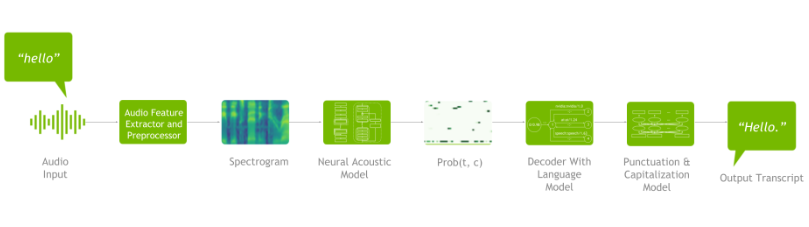
\includegraphics[width=0.8\textwidth]{Figure2.1.png}
    \caption{Deep Learning Speech Recognition Pipeline [4]}
    \label{fig:pipeline}
\end{figure}

\textbf{Data Preprocessing}

Data preprocessing is the first step in the pipeline. Techniques such as Fast Fourier Transformations (FFT) with windowing and normalization are commonly used. For instance, Figure \ref{fig:mel-spectrogram} shows the Mel Spectrogram of an audio recording.

\begin{figure}[ht]
    \centering
    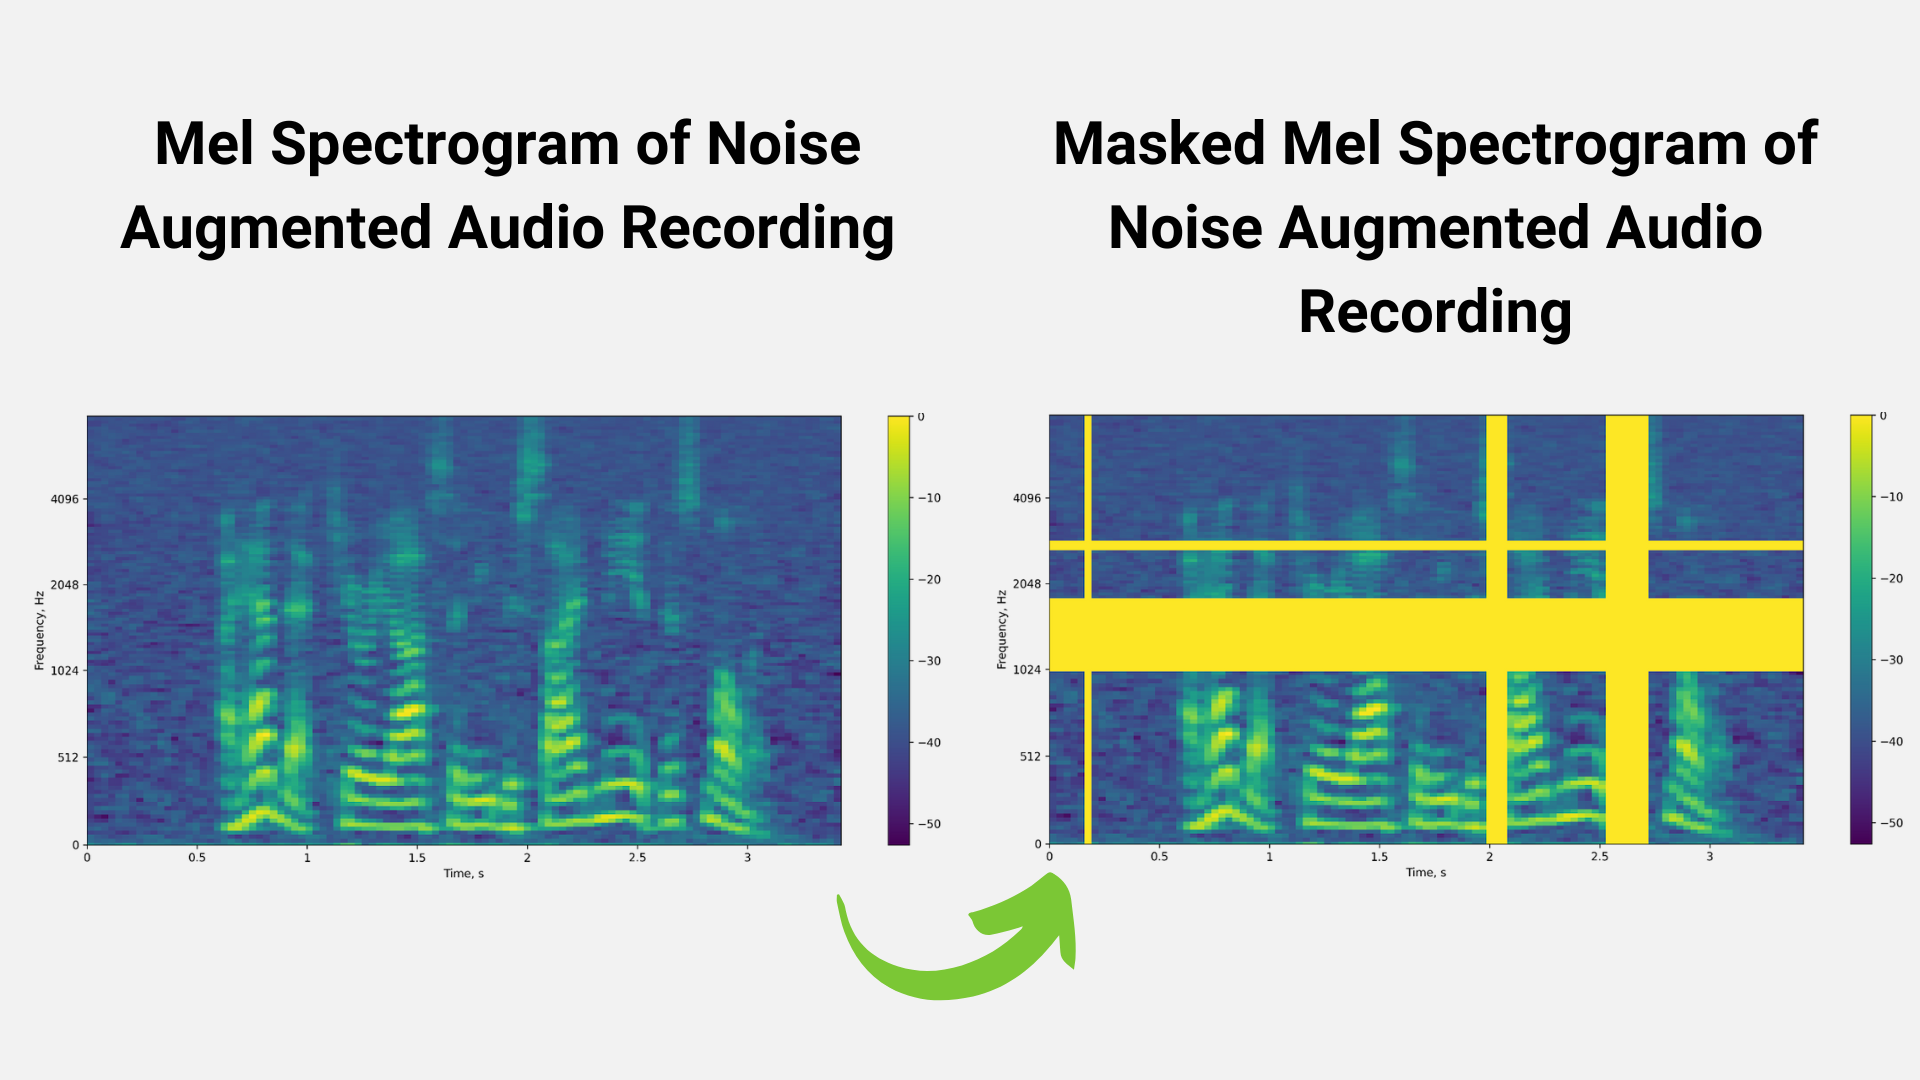
\includegraphics[width=0.8\textwidth]{Figure2.2.png}
    \caption{An audio recording: raw audio waveform (left) and mel spectrogram (right) [4]}
    \label{fig:mel-spectrogram}
\end{figure}

\textbf{Neural Acoustic Models}

Mel spectrograms are fed into the next stage: a Neural Acoustic Model. Examples include QuartzNet, CitriNet, ContextNet, Conformer-CTC, and Conformer-transducer. These models are crucial for addressing performance, accuracy, memory size, and computational costs.

\begin{figure}[ht]
    \centering
    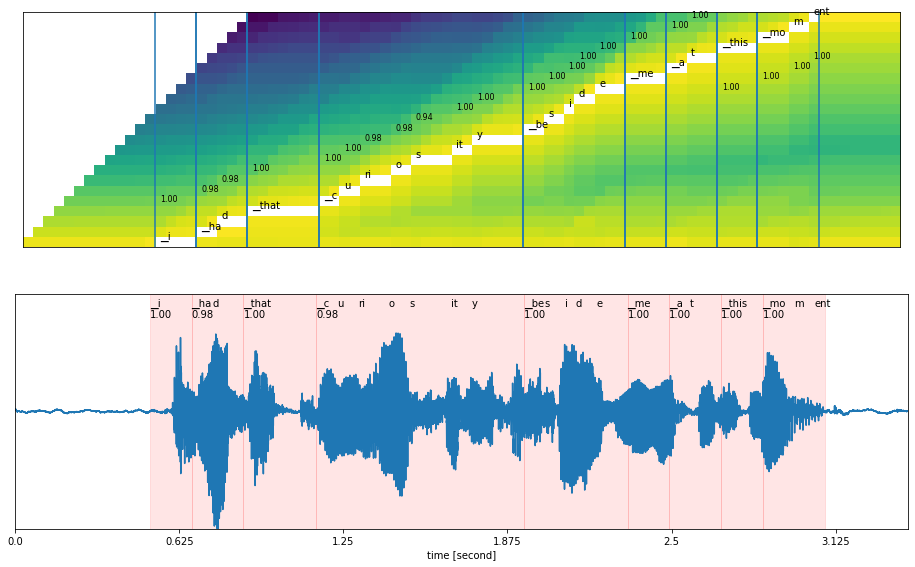
\includegraphics[width=0.8\textwidth]{Figure2.3.png}
    \caption{The acoustic model’s output includes a probabilistic distribution over vocabulary characters for each time step. [4]}
    \label{fig:acoustic-model-output}
\end{figure}

\textbf{Decoder and Language Model}

The acoustic model's output is fed into the decoder along with the language model. Decoders can be beam search or greedy decoders, and language models can be n-gram, KenLM, or neural scoring models.

\begin{figure}[ht]
    \centering
    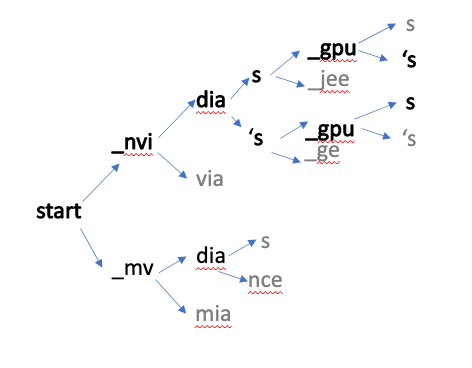
\includegraphics[width=0.8\textwidth]{Figure2.4.png}
    \caption{An example of a decoder workflow. [4]}
    \label{fig:decoder-workflow}
\end{figure}

\textbf{Punctuation and Capitalization Model}

The ASR pipeline generates text without punctuation or capitalization. A punctuation and capitalization model, often using BERT (Bidirectional Encoder Representations from Transformers), is used to improve text quality.

\begin{figure}[h]
    \centering
    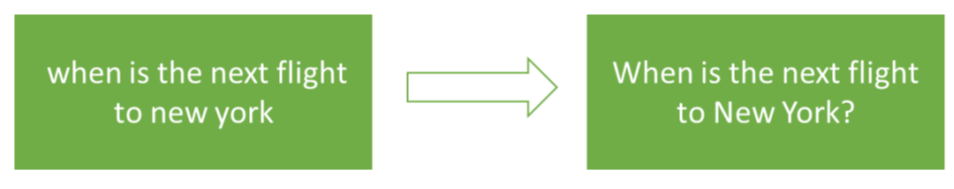
\includegraphics[width=0.8\textwidth]{Figure2.5.png}
    \caption{Example of a before-and-after punctuation and capitalization model. [4]}
    \label{fig:punctuation-model}
\end{figure}













    







\section*{Large Language Models the bases in Natural Language Processing and NLU}



\subsection{Natural Language Understanding}

Natural-language understanding (NLU), a subfield of natural-language processing in AI, focuses on machine reading comprehension. It's an AI-hard problem, drawing significant commercial interest due to applications in automated reasoning, machine translation, question answering, and more, including content analysis and voice-activated technologies.[8]



\subsection{Recurrent Neural Networks (RNN) for Sequence Modelling}

Recurrent Neural Networks (RNNs) are a type of AI specialized in processing sequential data, primarily used in Natural Language Processing and time series predictions. They maintain an internal memory, allowing them to remember previous inputs, a capability not found in standard neural networks. RNNs are distinctive for their feature of sharing weights across time, enabling them to incorporate historical information in computations. Their loss function and backpropagation are calculated at each time step [11].




Sequence modeling predicts the next entity in a sequence (like words or letters) based on prior entities. It employs specialized algorithms like RNN, LSTM, and Transformers, as conventional ANNs and CNNs are unsuitable for such tasks due to independent outputs, fixed-length inputs, and non-sharable parameters. RNN, a key algorithm, chains multiple ANNs to track and memorize past inputs, sharing weights and biases across time steps [14].



\subsection{Transformer Architecture}



Transformer models are a type of neural network that excel in understanding context and meaning in sequential data, like words in a sentence. They utilize a technique known as attention or self-attention, which allows the model to consider how different parts of the data are related, even if they are not close to each other. This method was first introduced in a 2017 paper by Google.

These models are considered one of the most advanced and powerful in the field of machine learning, spearheading what is often referred to as transformer AI. This new wave of technology is characterized by significant advancements in AI capabilities.

In August 2021, Stanford researchers highlighted the importance of transformer models by labeling them as "foundation models." They stressed that these models have been instrumental in driving a paradigm shift in AI, with their vast scale and scope expanding the boundaries of what was previously thought possible in the field [17]. \\


\textbf{What can transformer models do?}


Neural networks process language by generating vector-space representations of words or parts of words, considering the context to understand meaning. Recurrent Neural Networks (RNNs) have been commonly used for tasks like translation, processing language in a sequential manner. However, RNNs face challenges due to their sequential nature, which requires multiple steps to understand context, especially when words are far apart. This makes learning difficult and limits their compatibility with parallel-processing devices like GPUs and TPUs.

Convolutional Neural Networks (CNNs) offer a less sequential approach but still struggle with distant word relationships. In contrast, the Transformer, a newer model, significantly improves on these limitations. It employs a self-attention mechanism that directly models relationships between all words in a sentence, regardless of distance. This allows the Transformer to understand context in fewer steps and more efficiently.

For instance, in the sentence “I arrived at the bank after crossing the river”, a Transformer can quickly discern that “bank” refers to a riverbank by directly relating it to “river”. It achieves this by calculating attention scores for each word, indicating how much each word should influence the representation of another. This process is applied in both the encoder, which reads the input sentence, and the decoder, which generates the output.

The Transformer's capability extends beyond translation. It excels in tasks like coreference resolution, where it correctly identifies the reference of pronouns in different contexts, a task that has traditionally been challenging for machine translation systems. This efficiency and accuracy in handling complex language tasks demonstrate why the Transformer model is a significant advancement in the field of natural language processing [15].




\section*{Topic Segmentation}

Topic segmentation is a process used in natural language processing (NLP) and text analysis to divide a text into segments, each focusing on a specific topic. This technique identifies shifts in topic or subject matter within a document, making it easier to understand and analyze large volumes of text. Topic segmentation is essential for tasks like summarizing documents, information retrieval, and enhancing readability. It employs algorithms that look for cues such as keywords, phrases, and linguistic patterns indicative of a topic change. Effective topic segmentation helps in organizing information coherently, improving both automated and human comprehension of complex textual data.  




\subsection*{Latent Semantic Analysis}

Latent Semantic Analysis (LSA) is a natural language processing method used to analyze the relationships between documents and their terms. It generates concepts related to both documents and terms, based on the principle that words with similar meanings often appear in similar texts. LSA involves creating a matrix of word counts across documents, with unique words as rows and documents as columns. Singular Value Decomposition (SVD) is then applied to this matrix to reduce its size while maintaining the similarity structure among the columns. Cosine similarity is used to compare documents, where values close to 1 indicate high similarity, and values near 0 suggest low similarity. LSA, patented in 1988 and also known as latent semantic indexing (LSI) in information retrieval contexts, was developed by Deerwester, Dumais, Furnas, Harshman, Landauer, Lochbaum, and Streeter. [5]


Latent Semantic Analysis (LSA) is a technique that breaks down text documents into components, each reflecting a different aspect of meaning. It views text as an idea with multiple perspectives, converting a document-term matrix (where rows are documents and columns are terms) into a table of latent concepts. For instance, in a political context, documents could cover topics like foreign policy, elections, and reform. LSA plots these topics and relevant terms in matrices, indicating the strength of association between documents and topics, and between terms and topics.

The process involves vectorization methods like TF-IDF, creating a document-topic matrix where each cell represents the document's association with a particular topic. Simultaneously, a term-topic matrix is formed, showing how terms relate to different topics. Terms common to all topics, like "prime minister," have scores across all categories, reflecting their relevance.

LSA also identifies 'singular values', quantifying the significance of each topic in the dataset. This highlights dominant topics and reveals if additional topics should be considered. For example, a low value for 'reform' might indicate its lesser relevance compared to 'foreign policy' and 'elections', or the need for more topics like 'economics'.

Finally, LSA serves as a dimensionality reduction technique. From a large document-term matrix, it distills the essence into fewer topics, discarding less important data and focusing on the most significant topics. This results in a more compact representation of text, emphasizing themes over individual words.[6]

\subsection*{Topic Models: Probabilistic Models}


Probabilistic topic models are algorithms designed to uncover hidden thematic structures in large document collections. This article reviews the core concepts of this field, surveys current advancements, and explores future directions. The simplest topic model, Latent Dirichlet Allocation (LDA), and its connections to probabilistic modeling are discussed, along with algorithms for topic discovery. The article then examines research extending topic models, such as incorporating metadata, applying models to diverse data types like social networks, images, and genetics, and relaxing LDA's statistical assumptions.

The authors also highlight unexplored areas in topic modeling, emphasizing the need for rigorous model validation, innovative text and high-dimensional data visualization techniques, and applications beyond traditional information engineering to more scientific purposes. As digital storage of diverse knowledge forms like news, blogs, web pages, and scientific articles grows, the difficulty of finding relevant information increases. Topic modeling offers new computational tools to help organize, search, and understand these vast information troves. Instead of relying solely on keyword searches and links, topic modeling allows thematic exploration of documents, enabling users to "zoom in" and "zoom out" on specific or broader themes, understand their evolution over time, and see their interconnections. This thematic structure offers a new way to navigate and digest large information collections, surpassing human annotation's scalability.   [7]

\subsection*{Latent Dirichlecht Allocation}


Latent Dirichlet Allocation (LDA) is a fundamental technique in natural language processing, functioning as a Bayesian network and a generative statistical model. It operates on the principle of uncovering hidden (unobserved) groups within a dataset, which helps explain similarities in different parts of the data. As a Bayesian topic model, LDA is particularly adept at handling collections of observations, such as words in documents. In this context, it attributes the presence of each word in a document to a specific topic belonging to that document. A key characteristic of LDA is that it assumes each document is composed of a limited number of these topics. This assumption allows LDA to efficiently categorize and understand large collections of text by identifying the underlying thematic structures within them.   

\begin{itemize}
    \item \textbf{Topic Modeling}: A method to discover hidden thematic structures in a large collection of texts. It identifies topics distributed across documents, where a topic is characterized by a distribution of words.
    \item \textbf{LDA Basics}: Assumes documents are mixtures of topics and topics are mixtures of words. It models each document as a combination of various topics, and each topic as a combination of various words.
\end{itemize} [9]

\textbf{Process of LDA}
\begin{enumerate}
    \item \textbf{Initialization}: Assigns each word in documents to a random topic, based on a Dirichlet distribution.
    \item \textbf{Iterative Refinement}: Adjusts assignments using Gibbs sampling or variational inference, focusing on:
    \begin{itemize}
        \item Prevalence of each word across topics.
        \item Prevalence of topics in each document.
    \end{itemize}
    \item The goal is to enhance topic-word and document-topic assignments.
\end{enumerate} [9]

\textbf{Dirichlet Distribution} \\
The "Dirichlet" in LDA refers to the Dirichlet distribution, used to model the distribution of topics in documents and words in topics.\\


\textbf{Outcome of LDA}
\begin{itemize}
    \item A list of topics identified from the documents, each represented as a set of words.
    \item For each document, a distribution of these topics.
\end{itemize} [9]



\subsection{Speech Recognition from Videos with Audio}






\section{Topic Segmentation Algorithms:}

\subsubsection{Text Tiling}

The \textbf{TextTiling} algorithm is a technique for segmenting texts into multi-paragraph units that represent subtopics. It's designed to break a text into coherent segments, each covering a specific topic. The process involves the following steps:

\begin{enumerate}
    \item \textbf{Tokenization:} The text is divided into tokens, typically words.
    \item \textbf{Lexical Score Determination:} Measures the similarity between blocks of text, using a window of about 20 tokens, calculating a score based on the frequency of shared words.
    \item \textbf{Gap Score Calculation:} Identifies potential boundaries between topics by looking for gaps in these scores. A significant drop in similarity suggests a topic boundary.
    \item \textbf{Boundary Identification:} Involves smoothing the gap scores and determining which gaps significantly indicate a topic shift.
    \item \textbf{Segmentation:} The text is segmented at the identified boundaries, with each segment representing a coherent subtopic.
\end{enumerate}

This algorithm is useful in natural language processing tasks like document summarization, information retrieval, and content organization. Its effectiveness depends on the text nature and the granularity of the topics.



\subsubsection{C99 Algorithm}


The \textbf{C99} algorithm is a method for topic segmentation in texts. It segments texts into coherent units representing different topics or subtopics. Here is how the C99 algorithm works:

\begin{enumerate}
    \item \textbf{Sentence Tokenization:} The text is divided into sentences, which are the basic units for segmentation.
    \item \textbf{Sentence Similarity Matrix Creation:} Constructs a similarity matrix for each pair of sentences, typically using cosine similarity.
    \item \textbf{Ranking Matrix Formation:} The similarity matrix is transformed into a ranking matrix, ranking the similarity scores in each row.
    \item \textbf{Segmentation Using Eigenvector Calculation:} Employs eigenvector calculation to determine how to segment the ranking matrix.
    \item \textbf{Determination of Segment Boundaries:} Based on the eigenvector calculations, the algorithm determines the boundaries of the segments.
    \item \textbf{Final Segmentation:} The text is segmented at the identified boundaries, each representing a coherent topic or subtopic.
\end{enumerate}

C99 uses linear algebra techniques, like eigenvectors, for segmentation. It is effective for handling larger documents and is used in natural language processing for summarization, topic tracking, and information retrieval. The segmentation quality varies based on the text nature and similarity measures.













\section*{Prompt Engineering and Generative Artificial Intelligence (GAI)}

\subsection{Generative Artificial Intelligence}


\section*{Summary: What is Generative AI?}

Generative AI is a technology that rapidly creates new content from various inputs like text, images, sounds, animation, and 3D models. It operates through neural networks, recognizing patterns in data to produce original content. A key advancement in generative AI is the use of unsupervised or semi-supervised learning, allowing the utilization of large volumes of unlabeled data. This approach has led to the development of foundation models, which serve as the basis for AI systems capable of multiple tasks. Notable examples of foundation models are GPT-3 and Stable Diffusion. GPT-3, used in applications like ChatGPT, generates essays or other text-based content from brief prompts. Meanwhile, Stable Diffusion creates photorealistic images from textual descriptions. These developments showcase generative AI's versatility and its growing influence in various sectors, enabling more efficient and creative use of data.



\section*{Summary: What is Generative AI?}

Generative AI is a technology that rapidly creates new content from various inputs like text, images, sounds, animation, and 3D models. It operates through neural networks, recognizing patterns in data to produce original content. A key advancement in generative AI is the use of unsupervised or semi-supervised learning, allowing the utilization of large volumes of unlabeled data. This approach has led to the development of foundation models, which serve as the basis for AI systems capable of multiple tasks. Notable examples of foundation models are GPT-3 and Stable Diffusion. GPT-3, used in applications like ChatGPT, generates essays or other text-based content from brief prompts. Meanwhile, Stable Diffusion creates photorealistic images from textual descriptions. These developments showcase generative AI's versatility and its growing influence in various sectors, enabling more efficient and creative use of data.



\section*{Effective Learning Metrics for E-Learning Technologies}

\begin{enumerate}
    \item \textbf{Engagement Metrics:}
    \begin{itemize}
        \item Time on Task
        \item Course Login Frequency
        \item Participation in Discussions
    \end{itemize}

    \item \textbf{Performance Metrics:}
    \begin{itemize}
        \item Assessment Scores
        \item Progress Tracking
        \item Completion Rates
    \end{itemize}

    \item \textbf{Feedback and Self-Reporting Metrics:}
    \begin{itemize}
        \item Surveys and Questionnaires
        \item Self-Assessment Tools
    \end{itemize}

    \item \textbf{Behavioral Metrics:}
    \begin{itemize}
        \item Interaction with Learning Materials
        \item Use of Supplementary Resources
    \end{itemize}

    \item \textbf{Learning Analytics:}
    \begin{itemize}
        \item Predictive Analytics
        \item Adaptive Learning Metrics
    \end{itemize}

    \item \textbf{Satisfaction and Retention Metrics:}
    \begin{itemize}
        \item Net Promoter Score (NPS)
        \item Retention Rates
    \end{itemize}

    \item \textbf{Technology Interaction Metrics:}
    \begin{itemize}
        \item Platform Usability
        \item Device Usage Data
    \end{itemize}

    \item \textbf{Skill and Competency Development:}
    \begin{itemize}
        \item Pre- and Post-Tests
        \item Application of Skills
    \end{itemize}
\end{enumerate}



